% !TeX spellcheck = en_GB
\documentclass[12pt]{article}

\usepackage[top=1in, bottom=1in, left=1.25in, right=1.25in]{geometry}

%\usepackage[backend=biber, natbib=true, style=numeric, sorting=none]{biblatex}
\usepackage[sorting=none]{biblatex}
\bibliography{extended-essay}
%\usepackage[nottoc,numbib]{tocbibind}

\usepackage{hyperref} % clickable table of contents
\hypersetup{ % makes the clickable links in table of contents black
	colorlinks,
	citecolor=black,
	filecolor=black,
	linkcolor=black,
	urlcolor=black
}

%\DefineBibliographyStrings{english}{ % is needed for references to show up in the table of contents
%	bibliography = {References},
%}

\usepackage{setspace}

\usepackage{mathtools}

\usepackage{pgfplots}
\usepackage{tikz}
\pgfplotsset{compat=1.15}

\usepackage{listings}
\definecolor{codegreen}{rgb}{0,0.6,0}
\definecolor{codegray}{rgb}{0.5,0.5,0.5}
\definecolor{codepurple}{rgb}{0.58,0,0.82}
\definecolor{backcolour}{rgb}{0.95,0.95,0.92}
\lstdefinestyle{codestyle}{
	backgroundcolor=\color{backcolour},   
	commentstyle=\color{codegreen},
	keywordstyle=\color{magenta},
	numberstyle=\tiny\color{codegray},
	stringstyle=\color{codepurple},
	basicstyle=\scriptsize,
	breakatwhitespace=false,         
	breaklines=true,                 
	captionpos=b,                    
	keepspaces=true,                 
	numbers=left,                    
	numbersep=5pt,                  
	showspaces=false,                
	showstringspaces=false,
	showtabs=false,                  
	tabsize=2
}

\usepackage[justification=centering]{caption}
\usepackage{longtable}
\usepackage{float}
\usepackage{graphicx}
\usepackage{subcaption}
\usepackage{verbatim} %comments

\newcommand{\researchQuestion}{``To what extent is the Google's new JPEG encoder Guetzli superior to libjpeg-turbo, mozjpeg, jpeg-recompress and jpegoptim in terms of encoding time, compression rate and image quality?''}

\begin{document}
\captionsetup[figure]{labelfont={bf},labelformat={default},labelsep=period}
\captionsetup[table]{labelfont={bf},labelformat={default},labelsep=period}
\begin{titlepage}
	{\centering
	{\phantom{a}\par}
	\vspace{2cm}
	{\Large\bfseries Computer Science Extended Essay\par}
	\vspace{1cm}
	{\Large Comparison of lossy JPEG file format image encoders libjpeg-turbo, mozjpeg, jpeg-recompress, jpegoptim and guetzli in terms of encoding time, compression rate and image quality\par}
	\vspace{0.5cm}
	{\large Word count: 3936\par}\par}
\end{titlepage}
\clearpage
\tableofcontents
\clearpage
\doublespacing
\section{Introduction}\label{introduction}
The Internet provides a platform for organisations, individuals, businesses and governments to easily send out information for a target audience. Portion of it reaches every user of the internet, whether in the form of a text, a video or an image. Very often one aids another, which is especially true for images. They help to illustrate texts, providing additional information, as well as dictate our choices of videos - we select videos partly based on thumbnails - summarizing images. Images are nearly on every webpage and with ever-improving technology, they are also advancing. In the last decade, pictures improved greatly in quality and resolution, but it came with a cost - an increase in file size. In fact, the image size in web pages has more than doubled in the last five years~\cite{httparchive}. As images are taking up more and more disk space, it is important to conserve limited storage space as well as save bandwidth, which makes web pages load faster. One of the ways of doing that is reducing the file size using compression. Many tools currently exist for the compression of images of the most common format - JPEG~\cite{httparchiveinteresting}.

One of the first tools used to compress JPEG images was libjpeg, published by the Independent JPEG Group in 1991. In the last years, several new compression tools have been created, some of which are based on libjpeg. This includes libjpeg-turbo, released in 2010, which employed several advanced techniques, greatly improving the performance of libjpeg. Mozjpeg, released in 2014 included even more functionality. The amount of compression tools available has increased even further with the release of jpeg-recompress and jpegoptim. With such amount of work being put into JPEG image compression, it seemed like there would be little to none room left for improvement.

This turned out not to be the case when recently Google announced the release of a new, open-source JPEG encoder Guetzli, which claims to ``create high quality JPEG images with file sizes 35\% smaller than currently available methods.''~\cite{guetzli}. This kind of claim seems very unreasonable, as it is quite a big margin from the prevalent JPEG compression libraries. However, if it is true, it is quite ground-breaking, because it greatly improves a task that was thought to be barely improvable.

The interest of examining this claim, combined with the global importance of this topic and my personal fondness of various services and tools developed by Google, lead me to the following research question: \textbf{\researchQuestion}.
\clearpage
\section{Background knowledge}
\subsection{Lossy versus lossless image compression} \label{losslesslossy} 
Digital data compression algorithms can be described in two ways: \textit{lossless compression} and \textit{lossy compression}. \textit{Lossless compression} means that a file, in my case an image, can be reconstructed from a compressed (shrunk in size) file with every bit being identical to the source file. Although \textit{lossless compression} is much more desirable, as it provides a compressed image with every pixel being identical to the original, it can only provide a tiny amount of compression. \textit{Lossy compression} is the opposite. It means that a file, reconstructed from a compressed file will not be bit-by-bit identical, but instead will only be close to the source image. At the expense of image quality degradation, much higher magnitudes of compression can be achieved~\cite{digitalimagecompression1995}. A term that describes compressed images, that are not bit-by-bit identical, but are identical for a human eye under normal viewing conditions is \textit{visually lossless}~\cite{DigitalImageCompressionTechniques}. It is important to note that this concept is somewhat subjective, so it must be used cautiously.
%sitas  jau visai neblogai parasytas
\subsection{JPEG}
JPEG is currently the most ubiquitous image compression algorithm. It was created in 1992 by the JPEG (Joint Photographic Experts Group) for continuous-tone, still-frame, monochrome and color image compression~\cite{DigitalImageCompressionTechniques}. It compresses an image using complex mathematical operations such as discrete cosine transform. Although JPEG has a lossless compression mode, it is rarely used and is supported by very few applications. Much more widely used are the lossy compression modes, which will be relevant in this work.

The JPEG standard describes a parameter of every image - JPEG quality level. It is a value in the range from 0 to 100. This value adjusts how much detail can be lost in the compression process, 0 being the highest compression, 100 being the lowest. This results in the quality of JPEG images, 0 being the lowest quality and 100 being the highest. Every compression library that is described in this paper allows the user to set a quality level an image will be compressed at.

Below are short descriptions of several currently available and widely adopted JPEG compression libraries.
%TC:ignore
\begin{comment}
A JPEG file is made up of two parts: a \textit{container} and a \textit{payload}. A \textit{payload} holds the essential part - the image. It does not contain any metadata (time and date information, camera settings, image resolution, thumbnail of the image, etc). The \textit{container} contains the payload as well as metadata and any data that is needed for a decoder to decode the image.

Both the \textit{payload} and the \textit{container} used to employ the ITU T.81 standard (the original JPEG standard published by the JPEG), however only the \textit{payload} of modern JPEG files still does. The \textit{container} defined by ITU T.81 standard was called JPEG Interchange Format (JIF). It is rarely used anymore, because certain aspects of encoding and decoding JPEG images with a JIF container were difficult to implement and unavailing. Present-day JPEG files usually use two types of containers: JFIF (JPEG File Interchange Format) and EXIF (Exchangeable Image File Format). JFIF is a more basic and minimal version of JIF. It solves the difficulties arising from use of JIF containers. JFIF is most common with images found of the internet. EXIF is a newer, more complex container. It has the ability to store various amounts of metadata. It is most common with images, that are taken with a digital camera. ~\cite{highPerformanceImages}
\end{comment}
%TC:endignore

\subsection{JPEG compression libraries}
\subsubsection{libjpeg} \label{libjpeg}
% paziureti wikipedijoje kad nesidubliutu per daug, nes informacija is https://www.wikiwand.com/en/Libjpeg#/History
Libjpeg, published by the Independent JPEG Group (IJG) in 1991, is one of the earliest libraries to implement the JPEG codec. Its goal was to ``promote universal
JPEG file compatibility''~\cite{tomlanejpeg9}. Because of it being open-source, it is the origin of many modern JPEG encoding libraries. After the release of version 6b in 1998, a new version 7 was only released in 2009 and it broke backwards application binary interface (ABI) compatibility and created ``nonstandard files that can't be read by standard implementations, including older libjpeg.''~\cite{tomlanejpeg9}. This, combined with new versions being released that were regarded inferior to existing ones, lead to the disbanding of the IJG. The current state of libjpeg is essentially an abandoned project, which is why it will not be evaluated in my research together with modern compression tools.
%TC:ignore
\begin{comment}
After the release of version 6b in 1998, simultaneously as the version 7 of libjpeg was being developed, a variation of the libjpeg library was started to be developed by Miyasaka Masaru. It implemented single instruction, multiple data (SIMD) optimizations, which were supposed to increase the encoding and decoding speed of JPEG images. Several other developers joined Miyasaka Masaru and a fork of libjpeg, called libjpeg-turbo, was released in 2010.
\end{comment}
%TC:endignore

\subsubsection{libjpeg-turbo} \label{libjpeg-turbo}
In 2010, a JPEG compression library libjpeg-turbo was released by Miyasaka Masaru using libjpeg as a foundation. Its goal was to implemented single instruction, multiple data (SIMD) optimizations, which were supposed to increase the encoding and decoding speed of JPEG images. On computer systems that are based on certain architectures, the creators of libjpeg-turbo claim that this tool will be two to six times faster than libjpeg at compressing and decompressing JPEG images~\cite{libjpeg-turbo}. Another advantage of libjpeg-turbo is that it implements backwards ABI compatibility which was broken in libjpeg versions 7 and above.
% galbut daugiau references? wiki geras puslapis (libjpeg), bet wiki necituoti geriau

\subsubsection{mozjpeg} \label{mozjpeg}
Mozjpeg is a JPEG compression tool released by Mozilla in 2014. It is a fork of libjpeg-turbo including more functionality. One of the additions was jpgcrush functionality. It is a script written in Perl programming language which improves the file size by checking the image which is being compressed against several different compression configurations~\cite{mozjpeg1}. Another feature that was implemented into mozjpeg is trellis quantization, which is a specific process of turning a set of large numbers into smaller ones. Smaller numbers take less space to store, thus quantization generates compression~\cite{HandbookofDataCompression}. In 2014 Facebook announced that they were testing mozjpeg to improve the compression of images on facebook.com as well as donating \$60,000 to further development of the tool~\cite{mozjpeg2}.

\subsubsection{jpeg-recompress} \label{jpeg-recompress}
Jpeg-recompress is an open-source JPEG compression tool included in the JPEG archive project, released in 2014. Its underlying library is mozjpeg~\cite{jpeg-archive}. However, it uses mathematical methods to determine the visual similarity between compressed and uncompressed images in order to optimize the compression algorithm to output an image which is the most visually lossless.

\subsubsection{jpegoptim} \label{jpegoptim}
Jpegoptim is a JPEG compression library, developed by Timo Kokkonen. It is based on the libjpeg library. It employs several advanced techniques, such as optimization of Huffman tables~\cite{jpegoptim}, which is a data compression method based on compressing repeating numbers. This allows for JPEG image compression with minimal loss of image quality.

\subsubsection{Guetzli} \label{guetzli}
Guetzli is an open-source JPEG compression library released by Google in 2017. The creators claim that it creates ``high quality JPEG images with file sizes 35\% smaller than currently available methods''. It specifically targets the quantization process (compression of a set of values into a smaller set of smaller values) of JPEG compression, which often introduces the most visual loss of quality. It employs a search algorithm that tries to find the settings that produce the least visually different image that is of a significantly smaller file size~\cite{guetzli}. One clear disadvantage of Guetzli is that the search algorithm used takes a long time to find the optimal settings, thus the compression process takes a long time to complete.

\subsection{Image quality metrics} \label{imagequalitymetrics}
A way to calculate how much quality has a compressed image lost is to compare the original image with the processed one. To remove the element of subjectivity (which is introduced if image quality is judged by eye), mathematical models of image quality evaluation will be used for this task. Various algorithms quantifying the difference between two images exist. However, studies~\cite{qualityMetricEval1,qualityMetricEval2} show that the Visual Information Fidelity (VIF) and Multi-Scale Structural Similarity (MSSIM) image similarity indices are the most adequate to the human visual system, which is the way that human brains perceive images.

What is more, an image quality metric tool Butteraugli has recently been released by Google, which is based on the anatomy of the human eye~\cite{highPerformanceImages}. The Guetzli compression library has specifically been developed with the goal of scoring higher in Butteraugli~\cite{guetzli2}.
\clearpage
\section{Experiment}
\subsection{Methodology}
To find out the potential of the Guetzli compression, I will compare it against the following JPEG compression libraries:
\begin{itemize}
	\item \textbf{Libjpeg-turbo.} Built on top of libjpeg with the goal of being faster and better at compressing images than libjpeg.
	\item \textbf{Mozjpeg.} A fork of libjpeg-turbo, employing more advanced techniques to assist performance.
	\item \textbf{Jpeg-recompress.} Based on mozjpeg, it uses the visual similarity between compressed and uncompressed images in order to improve quality.
	\item \textbf{Jpegoptim.} Employs several advanced techniques in order to increase image quality.
\end{itemize}
I will measure several characteristics of each compressed image:
\begin{itemize}
	\item \textbf{Pixel encoding time.} I will be using the command-line utility ptime~\cite{ptime} in order to measure time taken to encode an image, which will be divided by the number of pixels to obtain the pixel encoding time (seconds per pixel).
	\item \textbf{Compression rate.} To compare the relative performance of different compression libraries between images, I will be calculating the reduction in bitrate (bits per pixel), which will be measured in percentage.
	\item \textbf{Image quality metrics.} I will be using VIF, MSSIM and Butteraugli image quality metric algorithms to evaluate the image quality. Although no scientific studies have yet been done on the evaluation of Butteraugli, I have decided to use it together with VIF and MSSIM for image quality analysis to see how it compares with already widely used tools and what scores will it assign for non-guetzli images.
\end{itemize}
To test the overall performance of compression libraries, a set of diverse images must be used. The set that I will be using will include images of two types, which will have certain subtypes:
\begin{itemize}
	\item \textbf{Real images.} Real-life images, which will be referred to as ``Real images'' in this paper.
		\begin{itemize}
			\item \textbf{Images of contrasting colours.} Images that include high contrast between black and white, as well as between other colours.
			\item \textbf{Highly colourful image.} Image consisting of many colours.
			\item \textbf{Light and dark images.} Images taken in a dark or light settings.
			\item \textbf{Black-and-white image.} Image with only black and white colours\footnote{\label{footnote1}A black-and-white image is used instead of a grayscale image, because Guetzli does not accept grayscale JPEG's as input.}.
			\item \textbf{Regular photograph.} Regular photo with no distinctive attributes.
		\end{itemize}
	\item \textbf{Non-real images.} Computer graphics or non-real-life images, which will be referred to as ``Non-real images'' in this paper.
		\begin{itemize}
			\item \textbf{Randomly generated image.} An image consisting of randomly generated pixels.
			\item \textbf{Gradient image.} An image including shifts from one colour to another.
			\item \textbf{Black-and-white image.} Image with only black and white colours\footnote{See footnote \ref{footnote1}}.
			\item \textbf{Image of a text.} A screenshot of a paragraph of text.
			\item \textbf{Illustrations.} Images that were drawn using computer graphics editing software.
			\item \textbf{Pattern.} Image consisting of a repeating pattern.
		\end{itemize}
\end{itemize}
The full set of images together with the sources can be found in figure~\ref{imageMatrix} in appendix~\ref{appendixSampleImages}.

Before the experiment, my hypothesis about the results I expect to see is:
\begin{itemize}
	\item \textbf{Libjpeg-turbo} will have the fastest pixel encoding time, however a weak point will be the compression rate. This is mainly due to libjpeg-turbo not employing several advanced techniques that other libraries do, which allows better performance at the expense of compression rate. I also expect the image quality to be very good.
	\item \textbf{Mozjpeg} will have the best compression rate due to it using more advanced technology relative to other libraries. However, this will come at the expense of pixel encoding time, which will be quite lengthy. I also expect the image quality to range from average to very good.
	\item \textbf{Jpeg-recompress} will have a very good image quality, because it was specifically designed to output an image that is as visually lossless as possible. However, this will heavily increase the encoding time. I expect the compression rate to be average.
	\item \textbf{Jpegoptim} will have good compression rate and image quality. It will have a shorter pixel encoding time than average, because of it not using many advanced techniques.
	\item \textbf{Guetzli} will have the best compression rate which will come at the expense of the worst pixel encoding time. This is due to it being the most technologically advanced and complex. I also expect the image quality to be very good.
\end{itemize}
Every encoding process will follow a certain algorithm. Firstly, a Java code will be run (appendix~\ref{javacode}), which encodes each image with every encoding library at the JPEG quality level 84 and produces a comma-separated value file. It will consist of the name of the image, library it was encoded with, the JPEG quality setting, the filesize of the compressed image and the time it took to encode. Then, each of the images will be measured with image quality metrics Butteraugli, VIF and MSSIM. All of this data will be gathered into one file and then analysed.

Although compressed images on most websites tend to fluctuate around the JPEG quality level 75 (see figure 4 in~\cite{qualitymark}), I will be compressing every image at the JPEG quality level 84. This is because 84 is the lowest possible quality setting that Guetzli can be set to without editing the source code (which would be using the tool not as the developers intended).
\subsection{Tools}
\subsubsection{Hardware}
Since the focus of this work is measuring how different JPEG compression libraries perform relative to each other, using only one computer is acceptable. I will be conducting the experiment on my personal computer:
\begin{itemize}
	\item \textbf{CPU:} Intel Core i7 3770 @ 3.40 GHz
	\item \textbf{RAM:} 8.00 GB Dual-Channel DDR3 @ 665 MHz
	\item \textbf{Motherboard:} Gigabyte B75M-D3V
	\item \textbf{Graphics:} 512 MB ATI Radeon HD 3800 Series
	\item \textbf{Storage:} 1397 GB Western Digital WD15EARX-00ZUDB0 HDD
\end{itemize}
\clearpage
\subsubsection{Software}
The software that I will be using to complete the experiment:
\begin{itemize}
	\item \textbf{Operating System:} Windows 8.1 Pro 64-bit
	\item \textbf{Encoding libraries:} libjpeg-turbo, mozjpeg, jpegoptim, jpeg-archive, guetzli.
	\item \textbf{Image quality metrics:} Butteraugli, Visual Information Fidelity~\cite{VIFneed}, Multi-Scale Structural Similarity~\cite{MSSIMneed}.
	\item \textbf{Other:} Matlab (for running the code of VIF and MSSIM), ptime (for measuring the time it takes to encode images), ImageMagick (for converting the JPEG images to portable pixel maps, because libjpeg-turbo does not take JPEG images as input).
\end{itemize}
\clearpage
\section{Analysis}
A table, consisting of raw data both about uncompressed images and images compressed with each of the five libraries is available in appendix~\ref{rawdata}.
\subsection{Pixel encoding time}
The pixel encoding times were calculated taking the total time taken to encode one image and dividing it by the number of pixels in the image. The graph shows the average time to encode per pixel for all 15 sample images. Because these numbers ended up being very small, in the graph they are multiplied by $10^4$.
% --- START TPP*10000 ---
\begin{figure}[H]
	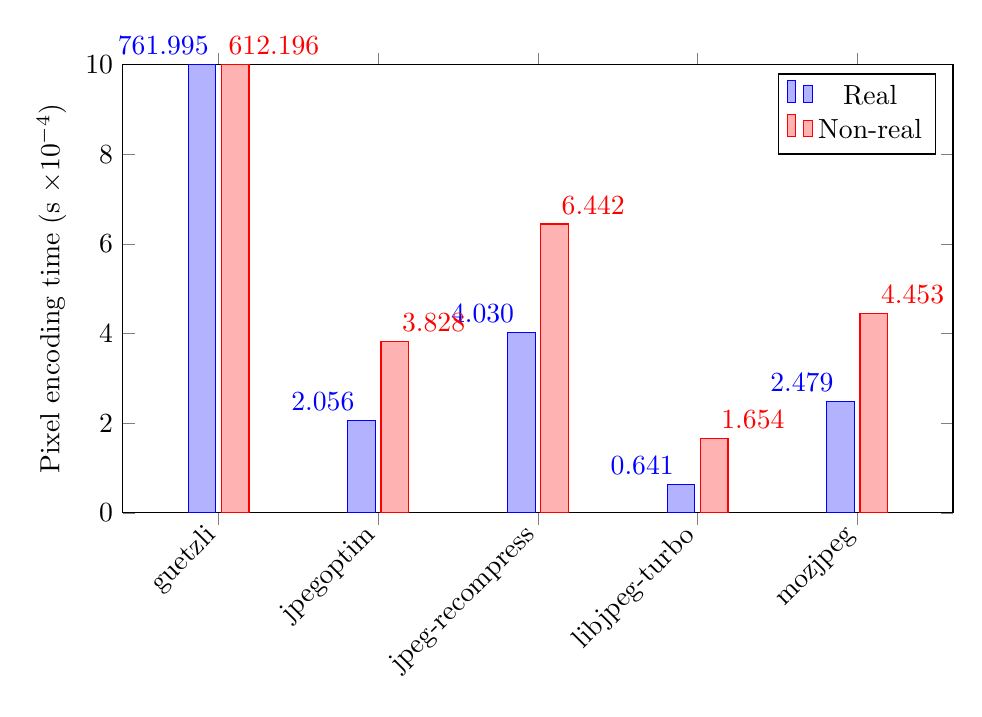
\begin{tikzpicture}
		\begin{axis}[
			ymin=0,
			%title=TPP*10000,
			/pgf/number format/.cd,
			1000 sep={},
			ybar,
			enlarge x limits=0.15,
			enlarge y limits=-0.15,
			%legend style={at={(0.5,-0.45)}, anchor=north, legend columns=-1},
			%legend style={at={(0.5,-0.45)}, anchor=north,},
			%ylabel={Time to encode per pixel $\times 10^4$ (s $\times 10^{-4}$)},
			ylabel={Pixel encoding time (s $\times 10^{-4}$)},
			symbolic x coords={guetzli,jpegoptim,jpeg-recompress,libjpeg-turbo,mozjpeg},
			xtick=data,
			nodes near coords,
			point meta=explicit symbolic,
			nodes near coords align={vertical},
			xticklabel style={rotate=45, anchor=east, align=center},
			width=\textwidth,
			height=\axisdefaultheight,
			restrict y to domain*=0:10,
		]
		\addplot+[every node near coord/.append style={xshift=-14pt}] coordinates {(guetzli,761.995)[\textcolor{blue}{761.995}] (jpegoptim,2.056)[\textcolor{blue}{2.056}] (jpeg-recompress,4.030)[\textcolor{blue}{4.030}] (libjpeg-turbo,0.641)[\textcolor{blue}{0.641}] (mozjpeg,2.479)[\textcolor{blue}{2.479}]};
		\addplot+[every node near coord/.append style={xshift=14pt}] coordinates {(guetzli,612.196)[\textcolor{red}{612.196}] (jpegoptim,3.828)[\textcolor{red}{3.828}] (jpeg-recompress,6.442)[\textcolor{red}{6.442}] (libjpeg-turbo,1.654)[\textcolor{red}{1.654}] (mozjpeg,4.453)[\textcolor{red}{4.453}]};
		\legend{Real,Non-real};
		\end{axis}
	\end{tikzpicture}
	\caption{The average pixel encoding time of JPEG compression libraries.}
	\label{avgCompressionSpeeds}
\end{figure}
% --- END TPP*10000 ---
Figure~\ref{avgCompressionSpeeds} shows that libjpeg-turbo was the fastest at encoding both real and non-real images. On average, it was 2.5 times faster than the second best performer - jpegoptim. The third fastest encoding library turned out to be mozjpeg, although it performed very similarly to jpegoptim. The fourth fastest encoder is jpeg-recompress. It was roughly 4.5 times slower than libjpeg-turbo and 1.5 times slower than the third fastest mozjpeg.

The slowest library was guetzli. Although I expected it to be slow, the results are still very surprising. On average, it was 200 times slower than the next-slowest library (mozjpeg) and almost 600 times slower than the fastest (libjpeg-turbo). This creates serious doubt about the feasibility of guetzli.

In the real image category, the image \textit{plane.jpg} stood out - all libraries apart from mozjpeg and guetzli took significantly longer to encode it compared to other images (see appendix~\ref{appendixEncodingSpeed}). I believe this is because of the amount of detail in the image - there are many clouds, which create a granular image (see figure~\ref{planeCutout}).
\begin{figure}[H]
	\centering
	\includegraphics[trim={9cm 10cm 9cm 20cm},clip,scale=0.6]{plane.jpg}
	\caption{A full of details part of the image \textit{plane.jpg}.}
	\label{planeCutout}
\end{figure}
In the non-real image category, the \textit{randomimage.jpg} image stood out - on average, it had a significantly longer pixel encoding time compared to other images (see appendix~\ref{appendixEncodingSpeed}). This is reasonable - compressing an image consisting of completely random pixels that do not have common features is a complex task, which lengthens the encoding process.

All of the compression libraries (except guetzli) show a trend of non-real images taking longer to compress than real images. This was unexpected, because real world images seem to be more complex in terms of colour and details. A possible cause for such results is compression libraries being optimized for the task of complex real-world image encoding. This is reasonable, because such images usually take up more space than computer graphics, making them more common targets for compression.
\subsection{Compression rate}
The compression rate was calculated by dividing the difference in bitrate between the raw and compressed images from the bitrate of the raw image. Figure~\ref{avgCompressionRate} shows the average compression rates of different libraries.
% --- START BPP ---
\begin{figure}[H]
	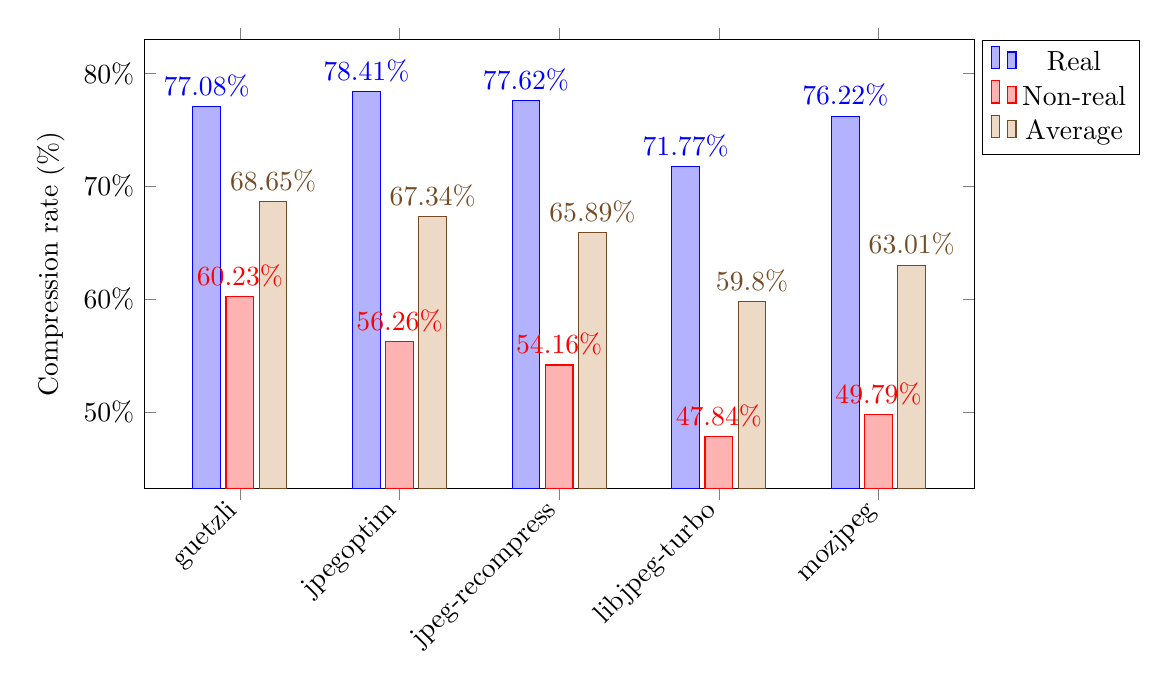
\begin{tikzpicture}
		\begin{axis}[
			/pgf/number format/.cd,
			1000 sep={},
			ybar,
			enlargelimits=0.15,
			%legend style={at={(0.5,-0.45)}, anchor=north, legend columns=-1},
			%legend style={at={(0.5,-0.45)}, anchor=north,},
			legend style={at={(1.2,1)},anchor=north east},
			ylabel={Compression rate (\%)},
			symbolic x coords={guetzli,jpegoptim,jpeg-recompress,libjpeg-turbo,mozjpeg},
			xtick=data,
			nodes near coords,
			nodes near coords align={vertical},
			xticklabel style={rotate=45, anchor=east, align=center},
			point meta={y*100},
			yticklabel = {\pgfmathparse{\tick*100}\pgfmathprintnumber{\pgfmathresult}\%},
			nodes near coords={\pgfmathprintnumber\pgfplotspointmeta\%},
			width=\textwidth,
			height=\axisdefaultheight,
		]
		\addplot coordinates {(guetzli,0.7708) (jpegoptim,0.7841) (jpeg-recompress,0.7762) (libjpeg-turbo,0.7177) (mozjpeg,0.7622)};
		\addplot coordinates {(guetzli,0.6023) (jpegoptim,0.5626) (jpeg-recompress,0.5416) (libjpeg-turbo,0.4784) (mozjpeg,0.4979)};
		\addplot coordinates {(guetzli,0.68655) (jpegoptim,0.67335) (jpeg-recompress,0.6589) (libjpeg-turbo,0.59805) (mozjpeg,0.63005)};
		\legend{Real,Non-real,Average};
		\end{axis}
	\end{tikzpicture}
	\caption{The average compression rate of JPEG compression libraries.}
	\label{avgCompressionRate}
\end{figure}
% --- END BPP ---
Libjpeg-turbo achieved the lowest average compression rate. This was expected, as libjpeg-turbo lacks the advanced techniques present in other compression libraries. Surprisingly, second to worst compression was achieved using mozjpeg. I expected it to perform better, considering its use of advanced techniques. Jpeg-recompress had the third-best compression rate, performing slightly worse than the second and first-best: jpegoptim and guetzli. Overall, the differences in compression rates between different libraries are very slight. On average, the best compression rate (guetzli) was only roughly 15\% better than the worst (libjpeg-turbo).

While the differences in compression rates, achieved by the libraries in the real image category are minimal, they are larger in the non-real images. Guetzli achieved 7\% better compression rates than the second-best jpegoptim and 25\% better than the worst libjpeg-turbo.

Developers of guetzli claim, that it creates ``JPEG images with file sizes 35\% smaller than currently available methods''~\cite{guetzli}. There is no doubt that guetzli achieved the best compression rates using my sample image set. However, the overall compression rate of guetzli was only 7\% better than the other four tools (libjpeg-turbo, mozjpeg, jpeg-recompress, jpegoptim) examined (1\% using real images, 16\% using non-real images).

In the non-real image category, the image \textit{randomimage.jpg} stood out. The average compression rate of it was only 4.4\% (see appendix~\ref{appendixCompressionRate}), which is very small compared to other images, some of which reached up to 90\% compression rates. Jpeg-recompress did not compress the image at all, outputting an error which informs that the output filesize would be larger than the original filesize (achieving a negative compression rate). Mozjpeg and libjpeg-turbo tried to compress it, failing and producing even larger files, respectively achieving -11.96\% and -2.92\% compression rates (see figures~\ref{jpeg-recompressNonRealCompressionRate},~\ref{libjpeg-turboNonRealCompressionRate} and~\ref{mozjpegNonRealCompressionRate} in appendix~\ref{appendixCompressionRate}).
\subsection{Image quality}
I used three different image quality metrics for the image quality evaluation, however testing revealed some flaws. It turned out to be difficult to compare quality differences between images using the MSSIM index, because differences between image qualities were very slight (see appendix~\ref{rawdata}). Butteraugli seemed to be somewhat subjective, giving significantly better scores to images encoded with guetzli. Although this is somewhat reasonable (guetzli was developed to achieve better butteraugli scores), I have decided to use VIF as the measure of image quality. It seemed to be the most objective measure, which best represents the quality of image. Not only did it not seem to favour a certain library, but it also produced more diverse results, which helps highlighting differences between JPEG encoding libraries.

Figure~\ref{avgImageQuality} shows the average image quality of images, compressed with different libraries.
% --- START VIF ---
\begin{figure}[H]
	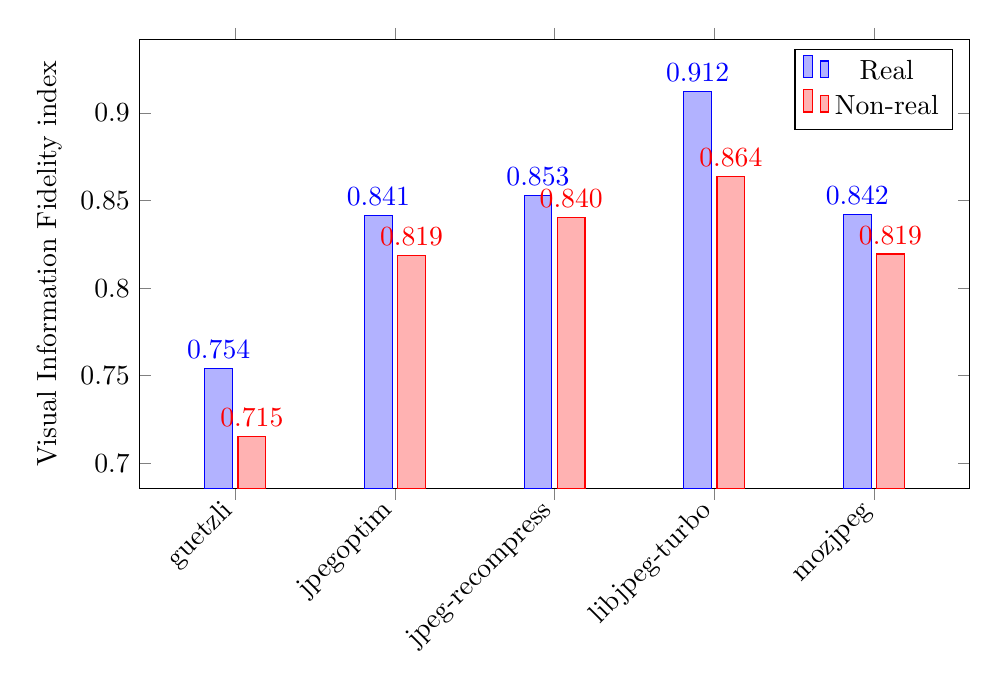
\begin{tikzpicture}
		\begin{axis}[
			/pgf/number format/.cd,
			1000 sep={},
			ybar,
			enlargelimits=0.15,
			%legend style={at={(0.5,-0.45)}, anchor=north, legend columns=-1},
			%legend style={at={(0.5,-0.45)}, anchor=north,},
			ylabel={Visual Information Fidelity index},
			symbolic x coords={guetzli,jpegoptim,jpeg-recompress,libjpeg-turbo,mozjpeg},
			xtick=data,
			nodes near coords={\pgfmathprintnumber[fixed zerofill, precision=3]{\pgfplotspointmeta}},
			nodes near coords align={vertical},
			xticklabel style={rotate=45, anchor=east, align=center},
			width=\textwidth,
			height=\axisdefaultheight,
		]
		\addplot coordinates {(guetzli,0.754232) (jpegoptim,0.841332) (jpeg-recompress,0.852836) (libjpeg-turbo,0.91227) (mozjpeg,0.842074)};
		\addplot coordinates {(guetzli,0.715392) (jpegoptim,0.818763) (jpeg-recompress,0.840332) (libjpeg-turbo,0.863908) (mozjpeg,0.819485)};
		\legend{Real,Non-real};
		\end{axis}
	\end{tikzpicture}
	\caption{The average image quality of JPEG compression libraries.}
	\label{avgImageQuality}
\end{figure}
% --- END VIF ---
Libjpeg-turbo managed to achieve the best image quality both in real and non-real image categories, which was expected. The second best performing library was jpeg-recompress, which is also unsurprising, because it is designed to compress images as visually lossless as possible. The third and fourth-best performers are mozjpeg and jpegoptim, both of which performed very similarly. The lowest quality was achieved by guetzli. Overall, all of the libraries performed very similarly, with only libjpeg-turbo achieving a slightly higher and guetzli - slightly lower VIF index.

Guetzli achieving the lowest average image quality is very unforeseen. With it being so technologically advanced, I expected only the encoding time to be a trade-off. It performed 12\% worse than the overall average and 20\% worse than the best-performer libjpeg-turbo.

Overall, compressed non-real images of every encoding library were of lower quality than real images. One image that stood out in the non-real image category was \textit{gradient.jpg} (figure~\ref{gradientImage}).
\begin{figure}[H]
	\centering
	\includegraphics[scale=0.5]{gradient.jpg}
	\caption{Sample image \textit{gradient.jpg}.}
	\label{gradientImage}
\end{figure}
It consistently achieved poorer than average image qualities by up to 60\%. I believe this is because the image does not have any regions of uniform colour. The pixel colour changes both along the vertical and horizontal directions, making any compression result in big loss of data and a significant drop in image quality.
\clearpage
\section{Conclusion}
The best encoding library is the one that manages to achieve highest image quality with the highest compression rate while keeping the encoding times as short as possible. This is a very complex task, as attempts to achieve a higher compression rate involve the usage of advanced techniques that usually increase the encoding times and decrease the image quality.

In the experiment that I conducted, the JPEG encoding libraries performed mostly the way I expected them to.

\textbf{Libjpeg-turbo} performed as I hypothesised - it was the fastest library to encode images. This is normal, because it lacks the use of advanced techniques compared to other libraries. However, as expected, it had a poor compression rate. This allowed libjpeg-turbo to achieve a great image quality.

\textbf{Mozjpeg} did not have the greatest compression rate, and had a lengthy encoding time due to the advanced techniques employed. The image quality, as predicted, was above average.

\textbf{Jpeg-recompress} performed according to the hypothesis - it had a lenghty encoding time, which allowed it to achieve a very good compression rate and image quality, which is what jpeg-recompress was designed to accomplish.

\textbf{Jpegoptim} had a short encoding time, together with quite average compression rate and image quality. This was expected, because it does not use advanced techniques.

\textbf{Guetzli} did not perform as expected. Although it did have the best compression rate, the claim of creating ``35\% smaller''~\cite{guetzli} images compared to other methods was inaccurate. This number is much smaller - using my set of sample images, it was only 7\%. I expected the images to be very high quality, yet the experiment showed the opposite - guetzli-compressed images had the lowest overall quality. What is more, guetzli had 200 to 600 times longer encoding times than currently adopted methods. These three aspects combined help answer my research question - \researchQuestion. Guetzli is superior in terms of compression rate, however the advantage is slight and the tremendously lenghty encoding times and lower image quality make guetzli overall inferior to currently adopted methods.
\clearpage
\section{Evaluation}
There are points for improvement in my research. I evaluated only one JPEG quality level and the results might differ using more levels for comparison. While a certain quality level will work better for one type of image, it may not work as well for another. What is more,~\cite{mixing} shows that higher compression rates with little image quality loss can be achieved when combining compression libraries, i.e. using the output image from one library as input for another. Such combinations could definitely be further research, extending my current essay. Furthermore, various academic work shows that higher compression rates can be achieved using new image file formats, such as WebP. While I only tested the most common image format - JPEG, evaluation of different formats is possible and would add depth to my current research. It would also be relevant, because WebP is being adopted quickly and the use of this format on internet websites is rapidly growing.

Another point for improvement is in the usage of image quality metrics. One of the metrics that I ended up not using was Butteraugli. It is a new tool (released in 2017) and because of that, no scientific studies evaluating its performance have yet been done. Assessment of this tool and the usage of it to judge image quality together with other quality metric tools is a point for improvement that could add depth to my current work.
\clearpage
%TC:ignore
\section{References}
{\setstretch{1.56}
\printbibliography[heading=none]
}
\clearpage
\section{Appendix}
\subsection{Sample images used for testing}\label{appendixSampleImages}
\begin{figure}[H]
	\begin{subfigure}[b]{0.26\textwidth}
		\includegraphics[width = 1.5in]{wintertrees.jpg}
		\caption{wintertrees.jpg}
	\end{subfigure}%
	\begin{subfigure}[b]{0.26\textwidth}
		\includegraphics[width = 1.5in]{autumntrees.jpg}
		\caption{autumntrees.jpg}
	\end{subfigure}%
	\begin{subfigure}[b]{0.26\textwidth}
		\includegraphics[width = 1.5in]{sunset.jpg}
		\caption{sunset.jpg}
	\end{subfigure}%
	\begin{subfigure}[b]{0.26\textwidth}
		\includegraphics[width = 1.5in]{poolballs.jpg}
		\caption{poolballs.jpg}
	\end{subfigure}
	
	\begin{subfigure}[b]{0.26\textwidth}
		\includegraphics[width = 1.5in]{umbrella.jpg}
		\caption{umbrella.jpg}
	\end{subfigure}%
	\begin{subfigure}[b]{0.26\textwidth}
		\includegraphics[width = 1.5in]{plane.jpg}
		\caption{plane.jpg}
	\end{subfigure}%
	\begin{subfigure}[b]{0.26\textwidth}
		\includegraphics[width = 1.5in]{nightshot.jpg}
		\caption{nightshot.jpg}
	\end{subfigure}%
	\begin{subfigure}[b]{0.26\textwidth}
		\includegraphics[width = 1.5in]{ducks.jpg}
		\caption{ducks.jpg}
	\end{subfigure}
	
	\begin{subfigure}[b]{0.26\textwidth}
		\includegraphics[width = 1.5in]{culturalcentre.jpg}
		\caption{culturalcentre.jpg}
	\end{subfigure}%
	\begin{subfigure}[b]{0.26\textwidth}
		\includegraphics[width = 1.5in]{randomimage.jpg}
		\caption{randomimage.jpg}
	\end{subfigure}%
	\begin{subfigure}[b]{0.26\textwidth}
		\includegraphics[width = 1.5in]{gradient.jpg}
		\caption{gradient.jpg}
	\end{subfigure}%
	\begin{subfigure}[b]{0.26\textwidth}
		\includegraphics[width = 1.5in]{lipsum.jpg}
		\caption{lipsum.jpg}
	\end{subfigure}
	
	\begin{subfigure}[b]{0.26\textwidth}
		\includegraphics[width = 1.5in]{dragon.jpg}
		\caption{dragon.jpg}
	\end{subfigure}%
	\begin{subfigure}[b]{0.26\textwidth}
		\includegraphics[width = 1.5in]{face.jpg}
		\caption{face.jpg}
	\end{subfigure}%
	\begin{subfigure}[b]{0.26\textwidth}
		\includegraphics[width = 1.5in]{rays.jpg}
		\caption{rays.jpg}
	\end{subfigure}
	\caption{The set of images used for testing.}
	\label{imageMatrix}
\end{figure}
The full quality images can be found at \url{https://github.com/mpoc/EE-sample-images}.

Sources of the images:

{\setstretch{1.2}
\begin{description}
	\item[(a), (b), (c), (f), (i)] Images from my personal archive.
	\item[(d)] Marco Verch, 2017, \textit{Pool ball set}, viewed January 2018,\\\textless https://www.flickr.com/photos/30478819@N08/37188154050/\textgreater. Licensed under CC BY 2.0 (	https://creativecommons.org/licenses/by/2.0/).
	\item[(e)] Bill Harrison, 2014, \textit{Protected}, viewed January 2018,\\\textless https://www.flickr.com/photos/bill\_harrison/13886342085/\textgreater. Licensed under CC BY 2.0 (https://creativecommons.org/licenses/by/2.0/).
	\item[(g)] Image Compression, 2007, \textit{nightshot\_iso\_100}, viewed January 2018,\\\textless http://imagecompression.info/test\_images/\textgreater.
	\item[(h)] Susanne Nilsson, 2013, \textit{Ducks}, viewed January 2018,\\\textless https://www.flickr.com/photos/infomastern/11128183215/\textgreater. Licensed under CC BY-SA 2.0 (https://creativecommons.org/licenses/by-sa/2.0/).
	\item[(j)] Generated using Java code adapted from https://www.dyclassroom.com/image-processing-project/how-to-create-a-random-pixel-image-in-java.
	\item[(k)] Image from my personal archive, created using image and photo editing software Paint.net.
	\item[(l)] A screenshot of the webpage https://loremipsumgenerator.com/.
	\item[(m)] Brandon James Scott, 2012, \textit{Dragon Scream}, viewed January 2018,\\\textless https://www.flickr.com/photos/brandonjamesscott/7591523382\textgreater. Licensed under CC BY-NC-ND 2.0 (https://creativecommons.org/licenses/by-nc-nd/2.0/).
	\item[(n)] Jarrett Kupcinski, 2011, \textit{JKPP luligirl}, viewed January 2018,\\\textless https://www.flickr.com/photos/kpcnsk/6377666717/\textgreater. Licensed under CC BY-NC 2.0 (https://creativecommons.org/licenses/by-nc/2.0/).
	\item[(o)] ASUNI N, GIACHETTI A, ``TESTIMAGES: A Large Data Archive For Display and Algorithm Testing'', Journal of Graphics Tools, Volume 17, Issue 4, 2015, pages 113-125, DOI:10.1080/2165347X.2015.1024298 AND ASUNI N, GIACHETTI A, ``TESTIMAGES: a large-scale archive for testing visual devices and basic image processing algorithms'', STAG - Smart Tools \& Apps for Graphics Conference, 2014.
\end{description}
}
\subsection{Java code for the image encoding}\label{javacode}
This Java code encodes each image with every encoding library and produces a comma-separated value file. It consists of the name of the image, library it was encoded with, the JPEG quality setting, the filesize of the compressed image and the time it took to encode. It also uses a batch file, the code of which can be found in section~\ref{batchcode}.

\lstset{style=codestyle}
{\setstretch{1.2}
	\lstinputlisting[language=Java]{encoding_script.java}
}

\subsection{Batch code for image encoding}\label{batchcode}
{\setstretch{1.2}
	\lstinputlisting[language=command.com]{encoding_script.bat}
}

\subsection{Raw data}\label{rawdata}
\begin{table}[H]
	\centering
	{\singlespacing
		\begin{tabular}{llllll}
			\hline
			Image          & Width (p) & Heigth (p) & Filesize (B) & Amount of pixels (p) & Bitrate (bpp) \\ \hline
			wintertrees    & 1024      & 1024       & 807290       & 1048576              & 6.1591               \\
			autumntrees    & 1536      & 1024       & 1469590      & 1572864              & 7.4747               \\
			sunset         & 1392      & 1044       & 745703       & 1453248              & 4.1050               \\
			poolballs      & 2048      & 1395       & 612246       & 2856960              & 1.7144               \\
			umbrella       & 2048      & 1246       & 938553       & 2551808              & 2.9424               \\
			plane          & 870       & 1160       & 712737       & 1009200              & 5.6499               \\
			nightshot      & 1568      & 1176       & 1055249      & 1843968              & 4.5782               \\
			culturalcentre & 1670      & 1253       & 1162019      & 2092510              & 4.4426               \\
			randomimage    & 640       & 320        & 123449       & 204800               & 4.8222               \\
			gradient       & 800       & 600        & 168763       & 480000               & 2.8127               \\
			lipsum         & 841       & 447        & 371117       & 375927               & 7.8976               \\
			dragon         & 900       & 720        & 169674       & 648000               & 2.0947               \\
			face           & 1024      & 791        & 192007       & 809984               & 1.8964               \\
			rays           & 1200      & 1200       & 1010142      & 1440000              & 5.6119               \\
			ducks          & 1536      & 1024       & 1118368      & 1572864              & 5.6883               \\ \hline
	\end{tabular}}
	\caption{Uncompressed image data.}
	\label{uncompressedData}
\end{table}
{\small
\setstretch{0.9} 
\begin{longtable}{llllll}
	\hline
	Image          & Compression tool & Filesize (B) & Time to encode (s) & VIF index & Bitrate (bpp) \\ \hline
	autumntrees    & guetzli          & 306219       & 187.805            & 0.76438   & 1.558                \\
	culturalcentre & guetzli          & 230245       & 146.926            & 0.77158   & 0.880                \\
	dragon         & guetzli          & 116243       & 35.701             & 0.74854   & 1.435                \\
	ducks          & guetzli          & 253115       & 86.872             & 0.77407   & 1.287                \\
	face           & guetzli          & 56207        & 34.035             & 0.79278   & 0.555                \\
	gradient       & guetzli          & 13716        & 12.351             & 0.54943   & 0.229                \\
	lipsum         & guetzli          & 88581        & 27.739             & 0.8436    & 1.885                \\
	nightshot      & guetzli          & 207319       & 200.636            & 0.75164   & 0.899                \\
	plane          & guetzli          & 146053       & 72.174             & 0.79171   & 1.158                \\
	poolballs      & guetzli          & 184423       & 163.516            & 0.70178   & 0.516                \\
	randomimage    & guetzli          & 85749        & 24.941             & 0.54426   & 3.350                \\
	rays           & guetzli          & 397698       & 70.419             & 0.81374   & 2.209                \\
	sunset         & guetzli          & 95345        & 97.183             & 0.69665   & 0.525                \\
	umbrella       & guetzli          & 316436       & 162.606            & 0.78442   & 0.992                \\
	wintertrees    & guetzli          & 211809       & 76.33              & 0.75186   & 1.616                \\
	autumntrees    & jpegoptim        & 274912       & 0.365              & 0.84037   & 1.398                \\
	culturalcentre & jpegoptim        & 208061       & 0.36               & 0.82909   & 0.795                \\
	dragon         & jpegoptim        & 123667       & 0.185              & 0.91922   & 1.527                \\
	ducks          & jpegoptim        & 275208       & 0.342              & 0.88679   & 1.400                \\
	face           & jpegoptim        & 47481        & 0.133              & 0.83159   & 0.469                \\
	gradient       & jpegoptim        & 20071        & 0.099              & 0.52968   & 0.335                \\
	lipsum         & jpegoptim        & 86683        & 0.14               & 0.8945    & 1.845                \\
	nightshot      & jpegoptim        & 160551       & 0.273              & 0.81916   & 0.697                \\
	plane          & jpegoptim        & 143285       & 0.362              & 0.86204   & 1.136                \\
	poolballs      & jpegoptim        & 160978       & 0.364              & 0.79924   & 0.451                \\
	randomimage    & jpegoptim        & 115365       & 0.197              & 0.90404   & 4.506                \\
	rays           & jpegoptim        & 364811       & 0.441              & 0.83355   & 2.027                \\
	sunset         & jpegoptim        & 98566        & 0.231              & 0.77025   & 0.543                \\
	umbrella       & jpegoptim        & 333615       & 0.411              & 0.90317   & 1.046                \\
	wintertrees    & jpegoptim        & 183602       & 0.288              & 0.86188   & 1.401                \\
	autumntrees    & jpeg-recompress  & 285923       & 0.722              & 0.85158   & 1.454                \\
	culturalcentre & jpeg-recompress  & 214873       & 0.722              & 0.83892   & 0.821                \\
	dragon         & jpeg-recompress  & 129258       & 0.383              & 0.92739   & 1.596                \\
	ducks          & jpeg-recompress  & 284668       & 0.692              & 0.89604   & 1.448                \\
	face           & jpeg-recompress  & 48759        & 0.372              & 0.83741   & 0.482                \\
	gradient       & jpeg-recompress  & 20409        & 0.402              & 0.53116   & 0.340                \\
	lipsum         & jpeg-recompress  & 89562        & 0.358              & 0.90286   & 1.906                \\
	nightshot      & jpeg-recompress  & 165787       & 0.591              & 0.82764   & 0.719                \\
	plane          & jpeg-recompress  & 148479       & 0.592              & 0.87235   & 1.177                \\
	poolballs      & jpeg-recompress  & 168460       & 0.857              & 0.82062   & 0.472                \\
	randomimage    & jpeg-recompress  & 123449       & 0.109              & 1         & 4.822                \\
	rays           & jpeg-recompress  & 376189       & 0.71               & 0.84317   & 2.090                \\
	sunset         & jpeg-recompress  & 101768       & 0.511              & 0.78053   & 0.560                \\
	umbrella       & jpeg-recompress  & 345090       & 0.884              & 0.91427   & 1.082                \\
	wintertrees    & jpeg-recompress  & 190406       & 0.501              & 0.87357   & 1.453                \\
	autumntrees    & libjpeg-turbo    & 360159       & 0.057              & 0.89653   & 1.832                \\
	culturalcentre & libjpeg-turbo    & 274083       & 0.08               & 0.88907   & 1.048                \\
	dragon         & libjpeg-turbo    & 145187       & 0.048              & 0.95339   & 1.792                \\
	ducks          & libjpeg-turbo    & 359221       & 0.093              & 0.92563   & 1.827                \\
	face           & libjpeg-turbo    & 59787        & 0.044              & 0.88665   & 0.591                \\
	gradient       & libjpeg-turbo    & 25040        & 0.052              & 0.58111   & 0.417                \\
	lipsum         & libjpeg-turbo    & 108716       & 0.113              & 0.91715   & 2.314                \\
	nightshot      & libjpeg-turbo    & 198518       & 0.096              & 0.87162   & 0.861                \\
	plane          & libjpeg-turbo    & 180483       & 0.191              & 0.90986   & 1.431                \\
	poolballs      & libjpeg-turbo    & 239023       & 0.077              & 0.98846   & 0.669                \\
	randomimage    & libjpeg-turbo    & 127053       & 0.084              & 0.91174   & 4.963                \\
	rays           & libjpeg-turbo    & 497130       & 0.065              & 0.93341   & 2.762                \\
	sunset         & libjpeg-turbo    & 129161       & 0.096              & 0.86694   & 0.711                \\
	umbrella       & libjpeg-turbo    & 396034       & 0.156              & 0.96275   & 1.242                \\
	wintertrees    & libjpeg-turbo    & 251257       & 0.05               & 0.89957   & 1.917                \\
	autumntrees    & mozjpeg          & 309897       & 0.494              & 0.84097   & 1.576                \\
	culturalcentre & mozjpeg          & 218041       & 0.456              & 0.82908   & 0.834                \\
	dragon         & mozjpeg          & 141741       & 0.269              & 0.92102   & 1.750                \\
	ducks          & mozjpeg          & 276752       & 0.438              & 0.88679   & 1.408                \\
	face           & mozjpeg          & 56043        & 0.166              & 0.83194   & 0.554                \\
	gradient       & mozjpeg          & 26496        & 0.102              & 0.53187   & 0.442                \\
	lipsum         & mozjpeg          & 91244        & 0.163              & 0.89484   & 1.942                \\
	nightshot      & mozjpeg          & 186152       & 0.383              & 0.82103   & 0.808                \\
	plane          & mozjpeg          & 153723       & 0.28               & 0.86208   & 1.219                \\
	poolballs      & mozjpeg          & 185846       & 0.514              & 0.79952   & 0.520                \\
	randomimage    & mozjpeg          & 138216       & 0.216              & 0.90368   & 5.399                \\
	rays           & mozjpeg          & 366246       & 0.505              & 0.83356   & 2.035                \\
	sunset         & mozjpeg          & 109331       & 0.297              & 0.77113   & 0.602                \\
	umbrella       & mozjpeg          & 394909       & 0.581              & 0.90619   & 1.238                \\
	wintertrees    & mozjpeg          & 186605       & 0.339              & 0.86188   & 1.424               \\ \hline
	\caption{Compressed image data.}
	\label{compressedData}
\end{longtable}}
Some data has been omitted from these tables to avoid redundancy. The full data of the experiment, including data for images, compressed with JPEG quality levels 87, 90 and 93, as well as MSSIM and Butteraugli indexes for every image can be found at \url{https://github.com/mpoc/EE-raw-data}.

\subsection{Additional graphs}
These graphs show processed data from every image with every compression library. There are references from the text to the graphs displayed below, however they are not necessary for the understanding of the work.
\newcommand{\heightOfDiagrams}{140pt}
\newcommand{\spaceBetweenDiagrams}{-0.7cm}
\subsubsection{Pixel encoding time}\label{appendixEncodingSpeed}
% ------------------------------------------------------------------------------------
\begin{figure}[H]
	\centering
	\begin{subfigure}{.5\textwidth}
		\centering
		\begin{tikzpicture}
		\begin{axis}[
		/pgf/number format/.cd,
		1000 sep={},
		ybar,
		enlargelimits=0.15,
		%legend style={at={(0.5,-0.45)}, anchor=north, legend columns=-1},
		ylabel style={align=center, text width=\heightOfDiagrams},
		ylabel={Pixel encoding time (s $\times 10^{-4}$)},
		symbolic x coords={autumntrees,culturalcentre,ducks,nightshot,plane,poolballs,sunset,umbrella,wintertrees},
		xtick=data,
		nodes near coords,
		nodes near coords align={vertical},
		every node near coord/.append style={rotate=90, anchor=west},
		xticklabel style={rotate=45, anchor=east, align=center},	
		width=\textwidth,
		%height=\axisdefaultheight,
		height=\heightOfDiagrams,
		]
		\addplot coordinates {(autumntrees,1194.032) (culturalcentre,702.152) (ducks,552.317) (nightshot,1088.067) (plane,715.161) (poolballs,572.343) (sunset,668.730) (umbrella,637.219) (wintertrees,727.940)};
		\end{axis}
		\end{tikzpicture}
		\caption{Real images.}
		\label{guetzliRealEncodingSpeed}
	\end{subfigure}%
	\begin{subfigure}{.5\textwidth}
		\centering
		\begin{tikzpicture}
		\begin{axis}[
		/pgf/number format/.cd,
		1000 sep={},
		ybar,
		enlargelimits=0.15,
		%legend style={at={(0.5,-0.45)}, anchor=north, legend columns=-1},
		ylabel style={align=center, text width=\heightOfDiagrams},
		%ylabel={\phantom{Time to encode per pixel $\times 10^4$ (s $\times 10^{-4}$)}},
		ylabel={\phantom{Pixel encoding time (s $\times 10^{-4}$)}},
		symbolic x coords={dragon,face,gradient,lipsum,randomimage,rays},
		xtick=data,
		nodes near coords,
		nodes near coords align={vertical},
		every node near coord/.append style={rotate=90, anchor=west},
		xticklabel style={rotate=45, anchor=east, align=center},
		width=\textwidth,
		%height=\axisdefaultheight,
		height=\heightOfDiagrams,
		]
		\addplot coordinates {(dragon,550.941) (face,420.193) (gradient,257.313) (lipsum,737.883) (randomimage,1217.822) (rays,489.021)};
		\end{axis}
		\end{tikzpicture}
		\caption{Non-real images.}
		\label{guetzliNonRealEncodingSpeed}
	\end{subfigure}
\caption{Image pixel encoding time of the guetzli library.}
\label{guetzliEncodingSpeed}
\end{figure}
\newgeometry{top=1cm,bottom=2cm}
{
\setlength{\abovecaptionskip}{4pt}
\begin{figure}[H]
	\centering
	\begin{subfigure}{.5\textwidth}
		\centering
		\begin{tikzpicture}
		\begin{axis}[
		/pgf/number format/.cd,
		1000 sep={},
		ybar,
		enlargelimits=0.15,
		%legend style={at={(0.5,-0.45)}, anchor=north, legend columns=-1},
		ylabel style={align=center, text width=\heightOfDiagrams},
		ylabel={Pixel encoding time (s $\times 10^{-4}$)},
		symbolic x coords={autumntrees,culturalcentre,ducks,nightshot,plane,poolballs,sunset,umbrella,wintertrees},
		xtick=data,
		nodes near coords,
		nodes near coords align={vertical},
		every node near coord/.append style={rotate=90, anchor=west},
		xticklabel style={rotate=45, anchor=east, align=center},
		width=\textwidth,
		%height=\axisdefaultheight,
		height=\heightOfDiagrams,
		]
		\addplot coordinates {(autumntrees,2.321) (culturalcentre,1.720) (ducks,2.174) (nightshot,1.481) (plane,3.587) (poolballs,1.274) (sunset,1.590) (umbrella,1.611) (wintertrees,2.747)};
		\end{axis}
		\end{tikzpicture}
		\caption{Real images.}
		\label{jpegoptimRealEncodingSpeed}
	\end{subfigure}%
	\begin{subfigure}{.5\textwidth}
		\centering
		\begin{tikzpicture}
		\begin{axis}[
		/pgf/number format/.cd,
		1000 sep={},
		ybar,
		enlargelimits=0.15,
		%legend style={at={(0.5,-0.45)}, anchor=north, legend columns=-1},
		ylabel style={align=center, text width=\heightOfDiagrams},
		ylabel={\phantom{Pixel encoding time (s $\times 10^{-4}$)}},
		symbolic x coords={dragon,face,gradient,lipsum,randomimage,rays},
		xtick=data,
		nodes near coords,
		nodes near coords align={vertical},
		every node near coord/.append style={rotate=90, anchor=west},
		xticklabel style={rotate=45, anchor=east, align=center},
		width=\textwidth,
		%height=\axisdefaultheight,
		height=\heightOfDiagrams,
		]
		\addplot coordinates {(dragon,2.855) (face,1.642) (gradient,2.063) (lipsum,3.724) (randomimage,9.619) (rays,3.063)};
		\end{axis}
		\end{tikzpicture}
		\caption{Non-real images.}
		\label{jpegoptimNonRealEncodingSpeed}
	\end{subfigure}
	\caption{Image pixel encoding time of the jpegoptim library.}
	\label{jpegoptimEncodingSpeed}
\end{figure}
\vspace{-1cm}
\begin{figure}[H]
	\centering
	\begin{subfigure}{.5\textwidth}
		\centering
		\begin{tikzpicture}
		\begin{axis}[
		/pgf/number format/.cd,
		1000 sep={},
		ybar,
		enlargelimits=0.15,
		%legend style={at={(0.5,-0.45)}, anchor=north, legend columns=-1},
		ylabel style={align=center, text width=\heightOfDiagrams},
		ylabel={Pixel encoding time (s $\times 10^{-4}$)},
		symbolic x coords={autumntrees,culturalcentre,ducks,nightshot,plane,poolballs,sunset,umbrella,wintertrees},
		xtick=data,
		nodes near coords,
		nodes near coords align={vertical},
		every node near coord/.append style={rotate=90, anchor=west},
		xticklabel style={rotate=45, anchor=east, align=center},
		width=\textwidth,
		%height=\axisdefaultheight,
		height=\heightOfDiagrams,
		]
		\addplot coordinates {(autumntrees,4.590) (culturalcentre,3.450) (ducks,4.400) (nightshot,3.205) (plane,5.866) (poolballs,3.000) (sunset,3.516) (umbrella,3.464) (wintertrees,4.778)};
		\end{axis}
		\end{tikzpicture}
		\caption{Real images.}
		\label{jpeg-recompressRealEncodingSpeed}
	\end{subfigure}%
	\begin{subfigure}{.5\textwidth}
		\centering
		\begin{tikzpicture}
		\begin{axis}[
		/pgf/number format/.cd,
		1000 sep={},
		ybar,
		enlargelimits=0.15,
		%legend style={at={(0.5,-0.45)}, anchor=north, legend columns=-1},
		ylabel style={align=center, text width=\heightOfDiagrams},
		ylabel={\phantom{Pixel encoding time (s $\times 10^{-4}$)}},
		symbolic x coords={dragon,face,gradient,lipsum,randomimage,rays},
		xtick=data,
		nodes near coords,
		nodes near coords align={vertical},
		every node near coord/.append style={rotate=90, anchor=west},
		xticklabel style={rotate=45, anchor=east, align=center},
		width=\textwidth,
		%height=\axisdefaultheight,
		height=\heightOfDiagrams,
		]
		\addplot coordinates {(dragon,5.910) (face,4.593) (gradient,8.375) (lipsum,9.523) (randomimage,5.322) (rays,4.931)};
		\end{axis}
		\end{tikzpicture}
		\caption{Non-real images.}
		\label{jpeg-recompressNonRealEncodingSpeed}
	\end{subfigure}
	\caption{Image pixel encoding time of the jpeg-recompress library.}
	\label{jpeg-recompressEncodingSpeed}
\end{figure}
\vspace{-1cm}
\begin{figure}[H]
	\centering
	\begin{subfigure}{.5\textwidth}
		\centering
		\begin{tikzpicture}
		\begin{axis}[
		/pgf/number format/.cd,
		1000 sep={},
		ybar,
		enlargelimits=0.15,
		%legend style={at={(0.5,-0.45)}, anchor=north, legend columns=-1},
		ylabel style={align=center, text width=\heightOfDiagrams},
		ylabel={Pixel encoding time (s $\times 10^{-4}$)},
		symbolic x coords={autumntrees,culturalcentre,ducks,nightshot,plane,poolballs,sunset,umbrella,wintertrees},
		xtick=data,
		nodes near coords,
		nodes near coords align={vertical},
		every node near coord/.append style={rotate=90, anchor=west},
		xticklabel style={rotate=45, anchor=east, align=center},
		width=\textwidth,
		%height=\axisdefaultheight,
		height=\heightOfDiagrams,
		]
		\addplot coordinates {(autumntrees,0.362) (culturalcentre,0.382) (ducks,0.591) (nightshot,0.521) (plane,1.893) (poolballs,0.270) (sunset,0.661) (umbrella,0.611) (wintertrees,0.477)};
		\end{axis}
		\end{tikzpicture}
		\caption{Real images.}
		\label{libjpeg-turboRealEncodingSpeed}
	\end{subfigure}%
	\begin{subfigure}{.5\textwidth}
		\centering
		\begin{tikzpicture}
		\begin{axis}[
		/pgf/number format/.cd,
		1000 sep={},
		ybar,
		enlargelimits=0.15,
		%legend style={at={(0.5,-0.45)}, anchor=north, legend columns=-1},
		ylabel style={align=center, text width=\heightOfDiagrams},
		ylabel={\phantom{Pixel encoding time (s $\times 10^{-4}$)}},
		symbolic x coords={dragon,face,gradient,lipsum,randomimage,rays},
		xtick=data,
		nodes near coords,
		nodes near coords align={vertical},
		every node near coord/.append style={rotate=90, anchor=west},
		xticklabel style={rotate=45, anchor=east, align=center},
		width=\textwidth,
		%height=\axisdefaultheight,
		height=\heightOfDiagrams,
		]
		\addplot coordinates {(dragon,0.741) (face,0.543) (gradient,1.083) (lipsum,3.006) (randomimage,4.102) (rays,0.451)};
		\end{axis}
		\end{tikzpicture}
		\caption{Non-real images.}
		\label{libjpeg-turboNonRealEncodingSpeed}
	\end{subfigure}
	\caption{Image pixel encoding time of the libjpeg-turbo library.}
	\label{libjpeg-turboEncodingSpeed}
\end{figure}

\begin{figure}[H]
	\centering
	\begin{subfigure}{.5\textwidth}
		\centering
		\begin{tikzpicture}
		\begin{axis}[
		/pgf/number format/.cd,
		1000 sep={},
		ybar,
		enlargelimits=0.15,
		%legend style={at={(0.5,-0.45)}, anchor=north, legend columns=-1},
		ylabel style={align=center, text width=\heightOfDiagrams},
		ylabel={Pixel encoding time (s $\times 10^{-4}$)},
		symbolic x coords={autumntrees,culturalcentre,ducks,nightshot,plane,poolballs,sunset,umbrella,wintertrees},
		xtick=data,
		nodes near coords,
		nodes near coords align={vertical},
		every node near coord/.append style={rotate=90, anchor=west},
		xticklabel style={rotate=45, anchor=east, align=center},
		width=\textwidth,
		%height=\axisdefaultheight,
		height=\heightOfDiagrams,
		]
		\addplot coordinates {(autumntrees,3.141) (culturalcentre,2.179) (ducks,2.785) (nightshot,2.077) (plane,2.774) (poolballs,1.799) (sunset,2.044) (umbrella,2.277) (wintertrees,3.233)};
		\end{axis}
		\end{tikzpicture}
		\caption{Real images.}
		\label{mozjpegRealEncodingSpeed}
	\end{subfigure}%
	\begin{subfigure}{.5\textwidth}
		\centering
		\begin{tikzpicture}
		\begin{axis}[
		/pgf/number format/.cd,
		1000 sep={},
		ybar,
		enlargelimits=0.15,
		%legend style={at={(0.5,-0.45)}, anchor=north, legend columns=-1},
		ylabel style={align=center, text width=\heightOfDiagrams},
		ylabel={\phantom{Pixel encoding time (s $\times 10^{-4}$)}},
		symbolic x coords={dragon,face,gradient,lipsum,randomimage,rays},
		xtick=data,
		nodes near coords,
		nodes near coords align={vertical},
		every node near coord/.append style={rotate=90, anchor=west},
		xticklabel style={rotate=45, anchor=east, align=center},
		width=\textwidth,
		%height=\axisdefaultheight,
		height=\heightOfDiagrams,
		]
		\addplot coordinates {(dragon,4.151) (face,2.049) (gradient,2.125) (lipsum,4.336) (randomimage,10.547) (rays,3.507)};
		\end{axis}
		\end{tikzpicture}
		\caption{Non-real images.}
		\label{mozjpegNonRealEncodingSpeed}
	\end{subfigure}
	\caption{Image pixel encoding time of the mozjpeg library.}
	\label{mozjpegEncodingSpeed}
\end{figure}
\vspace{-1cm}
% ------------------------------------------------------------------------------------
\subsubsection{Compression rate}\label{appendixCompressionRate}
% ------------------------------------------------------------------------------------
\vspace{-1cm}
\begin{figure}[H]
	\centering
	\begin{subfigure}{.5\textwidth}
		\centering
		\begin{tikzpicture}
		\begin{axis}[
		/pgf/number format/.cd,
		1000 sep={},
		ybar,
		enlargelimits=0.15,
		%legend style={at={(0.5,-0.45)}, anchor=north, legend columns=-1},
		ylabel={Compression rate (\%)},
		symbolic x coords={autumntrees,culturalcentre,ducks,nightshot,plane,poolballs,sunset,umbrella,wintertrees},
		xtick=data,
		nodes near coords,
		nodes near coords align={vertical},
		every node near coord/.append style={rotate=90, anchor=west},
		xticklabel style={rotate=45, anchor=east, align=center},
		point meta={y*100},
		yticklabel = {\pgfmathparse{\tick*100}\pgfmathprintnumber{\pgfmathresult}\%},
		nodes near coords={\pgfmathprintnumber\pgfplotspointmeta\%},
		width=\textwidth,
		%height=\axisdefaultheight,
		height=\heightOfDiagrams,
		]
		\addplot coordinates {(autumntrees,0.7916) (culturalcentre,0.8019) (ducks,0.7737) (nightshot,0.8035) (plane,0.7951) (poolballs,0.6988) (sunset,0.8721) (umbrella,0.6628) (wintertrees,0.7376)};
		\end{axis}
		\end{tikzpicture}
		\caption{Real images.}
		\label{guetzliRealCompressionRate}
	\end{subfigure}%
	\begin{subfigure}{.5\textwidth}
		\centering
		\begin{tikzpicture}
		\begin{axis}[
		/pgf/number format/.cd,
		1000 sep={},
		ybar,
		enlargelimits=0.15,
		%legend style={at={(0.5,-0.45)}, anchor=north, legend columns=-1},
		ylabel={\phantom{Compression rate (\%)}},
		symbolic x coords={dragon,face,gradient,lipsum,randomimage,rays},
		xtick=data,
		nodes near coords,
		nodes near coords align={vertical},
		every node near coord/.append style={rotate=90, anchor=west},
		xticklabel style={rotate=45, anchor=east, align=center},
		point meta={y*100},
		yticklabel = {\pgfmathparse{\tick*100}\pgfmathprintnumber{\pgfmathresult}\%},
		nodes near coords={\pgfmathprintnumber\pgfplotspointmeta\%},
		width=\textwidth,
		%height=\axisdefaultheight,
		height=\heightOfDiagrams,
		]
		\addplot coordinates {(dragon,0.3149) (face,0.7073) (gradient,0.9187) (lipsum,0.7613) (randomimage,0.3054) (rays,0.6063)};
		\end{axis}
		\end{tikzpicture}
		\caption{Non-real images.}
		\label{guetzliNonRealCompressionRate}
	\end{subfigure}
	\caption{Image compression rate of the guetzli library.}
	\label{guetzliCompressionRate}
\end{figure}
\vspace{-1cm}
\begin{figure}[H]
	\centering
	\begin{subfigure}{.5\textwidth}
		\centering
		\begin{tikzpicture}
		\begin{axis}[
		/pgf/number format/.cd,
		1000 sep={},
		ybar,
		enlargelimits=0.15,
		%legend style={at={(0.5,-0.45)}, anchor=north, legend columns=-1},
		ylabel={Compression rate (\%)},
		symbolic x coords={autumntrees,culturalcentre,ducks,nightshot,plane,poolballs,sunset,umbrella,wintertrees},
		xtick=data,
		nodes near coords,
		nodes near coords align={vertical},
		every node near coord/.append style={rotate=90, anchor=west},
		xticklabel style={rotate=45, anchor=east, align=center},
		point meta={y*100},
		yticklabel = {\pgfmathparse{\tick*100}\pgfmathprintnumber{\pgfmathresult}\%},
		nodes near coords={\pgfmathprintnumber\pgfplotspointmeta\%},
		width=\textwidth,
		%height=\axisdefaultheight,
		height=\heightOfDiagrams,
		]
		\addplot coordinates {(autumntrees,0.8129) (culturalcentre,0.8209) (ducks,0.7539) (nightshot,0.8479) (plane,0.7990) (poolballs,0.7371) (sunset,0.8678) (umbrella,0.6445) (wintertrees,0.7726)};
		\end{axis}
		\end{tikzpicture}
		\caption{Real images.}
		\label{jpegoptimRealCompressionRate}
	\end{subfigure}%
	\begin{subfigure}{.5\textwidth}
		\centering
		\begin{tikzpicture}
		\begin{axis}[
		/pgf/number format/.cd,
		1000 sep={},
		ybar,
		enlargelimits=0.15,
		%legend style={at={(0.5,-0.45)}, anchor=north, legend columns=-1},
		ylabel={\phantom{Compression rate (\%)}},
		symbolic x coords={dragon,face,gradient,lipsum,randomimage,rays},
		xtick=data,
		nodes near coords,
		nodes near coords align={vertical},
		every node near coord/.append style={rotate=90, anchor=west},
		xticklabel style={rotate=45, anchor=east, align=center},
		point meta={y*100},
		yticklabel = {\pgfmathparse{\tick*100}\pgfmathprintnumber{\pgfmathresult}\%},
		nodes near coords={\pgfmathprintnumber\pgfplotspointmeta\%},
		width=\textwidth,
		%height=\axisdefaultheight,
		height=\heightOfDiagrams,
		]
		\addplot coordinates {(dragon,0.2711) (face,0.7527) (gradient,0.8811) (lipsum,0.7664) (randomimage,0.0655) (rays,0.6389)};
		\end{axis}
		\end{tikzpicture}
		\caption{Non-real images.}
		\label{jpegoptimNonRealCompressionRate}
	\end{subfigure}
	\caption{Image compression rate of the guetzli library.}
	\label{jpegoptimCompressionRate}
\end{figure}

\begin{figure}[H]
	\centering
	\begin{subfigure}{.5\textwidth}
		\centering
		\begin{tikzpicture}
		\begin{axis}[
		/pgf/number format/.cd,
		1000 sep={},
		ybar,
		enlargelimits=0.15,
		%legend style={at={(0.5,-0.45)}, anchor=north, legend columns=-1},
		ylabel={Compression rate (\%)},
		symbolic x coords={autumntrees,culturalcentre,ducks,nightshot,plane,poolballs,sunset,umbrella,wintertrees},
		xtick=data,
		nodes near coords,
		nodes near coords align={vertical},
		every node near coord/.append style={rotate=90, anchor=west},
		xticklabel style={rotate=45, anchor=east, align=center},
		point meta={y*100},
		yticklabel = {\pgfmathparse{\tick*100}\pgfmathprintnumber{\pgfmathresult}\%},
		nodes near coords={\pgfmathprintnumber\pgfplotspointmeta\%},
		width=\textwidth,
		%height=\axisdefaultheight,
		height=\heightOfDiagrams,
		]
		\addplot coordinates {(autumntrees,0.8054) (culturalcentre,0.8151) (ducks,0.7455) (nightshot,0.8429) (plane,0.7917) (poolballs,0.7248) (sunset,0.8635) (umbrella,0.6323) (wintertrees,0.7641)};
		\end{axis}
		\end{tikzpicture}
		\caption{Real images.}
		\label{jpeg-recompressRealCompressionRate}
	\end{subfigure}%
	\begin{subfigure}{.5\textwidth}
		\centering
		\begin{tikzpicture}
		\begin{axis}[
		/pgf/number format/.cd,
		1000 sep={},
		ybar,
		enlargelimits=0.15,
		%legend style={at={(0.5,-0.45)}, anchor=north, legend columns=-1},
		ylabel={\phantom{Compression rate (\%)}},
		symbolic x coords={dragon,face,gradient,lipsum,randomimage,rays},
		xtick=data,
		nodes near coords,
		nodes near coords align={vertical},
		every node near coord/.append style={rotate=90, anchor=west},
		xticklabel style={rotate=45, anchor=east, align=center},
		point meta={y*100},
		yticklabel = {\pgfmathparse{\tick*100}\pgfmathprintnumber{\pgfmathresult}\%},
		nodes near coords={\pgfmathprintnumber\pgfplotspointmeta\%},
		width=\textwidth,
		%height=\axisdefaultheight,
		height=\heightOfDiagrams,
		]
		\addplot coordinates {(dragon,0.2382) (face,0.7461) (gradient,0.8791) (lipsum,0.7587) (randomimage,0.0000) (rays,0.6276)};
		\end{axis}
		\end{tikzpicture}
		\caption{Non-real images.}
		\label{jpeg-recompressNonRealCompressionRate}
	\end{subfigure}
	\caption{Image compression rate of the jpeg-recompress library.}
	\label{jpeg-recompressCompressionRate}
\end{figure}
\vspace{-1cm}
\begin{figure}[H]
	\centering
	\begin{subfigure}{.5\textwidth}
		\centering
		\begin{tikzpicture}
		\begin{axis}[
		/pgf/number format/.cd,
		1000 sep={},
		ybar,
		enlargelimits=0.15,
		%legend style={at={(0.5,-0.45)}, anchor=north, legend columns=-1},
		ylabel={Compression rate (\%)},
		symbolic x coords={autumntrees,culturalcentre,ducks,nightshot,plane,poolballs,sunset,umbrella,wintertrees},
		xtick=data,
		nodes near coords,
		nodes near coords align={vertical},
		every node near coord/.append style={rotate=90, anchor=west},
		xticklabel style={rotate=45, anchor=east, align=center},
		point meta={y*100},
		yticklabel = {\pgfmathparse{\tick*100}\pgfmathprintnumber{\pgfmathresult}\%},
		nodes near coords={\pgfmathprintnumber\pgfplotspointmeta\%},
		width=\textwidth,
		%height=\axisdefaultheight,
		height=\heightOfDiagrams,
		]
		\addplot coordinates {(autumntrees,0.7549) (culturalcentre,0.7641) (ducks,0.6788) (nightshot,0.8119) (plane,0.7468) (poolballs,0.6096) (sunset,0.8268) (umbrella,0.5780) (wintertrees,0.6888)};
		\end{axis}
		\end{tikzpicture}
		\caption{Real images.}
		\label{libjpeg-turboRealCompressionRate}
	\end{subfigure}%
	\begin{subfigure}{.5\textwidth}
		\centering
		\begin{tikzpicture}
		\begin{axis}[
		/pgf/number format/.cd,
		1000 sep={},
		ybar,
		enlargelimits=0.15,
		%legend style={at={(0.5,-0.45)}, anchor=north, legend columns=-1},
		ylabel={\phantom{Compression rate (\%)}},
		symbolic x coords={dragon,face,gradient,lipsum,randomimage,rays},
		xtick=data,
		nodes near coords,
		nodes near coords align={vertical},
		every node near coord/.append style={rotate=90, anchor=west},
		xticklabel style={rotate=45, anchor=east, align=center},
		point meta={y*100},
		yticklabel = {\pgfmathparse{\tick*100}\pgfmathprintnumber{\pgfmathresult}\%},
		nodes near coords={\pgfmathprintnumber\pgfplotspointmeta\%},
		width=\textwidth,
		%height=\axisdefaultheight,
		height=\heightOfDiagrams,
		]
		\addplot coordinates {(dragon,0.1443) (face,0.6886) (gradient,0.8516) (lipsum,0.7071) (randomimage,-0.0292) (rays,0.5079)};
		\end{axis}
		\end{tikzpicture}
		\caption{Non-real images.}
		\label{libjpeg-turboNonRealCompressionRate}
	\end{subfigure}
	\caption{Image compression rate of the libjpeg-turbo library.}
	\label{libjpeg-turboCompressionRate}
\end{figure}
\vspace{-1cm}
\begin{figure}[H]
	\centering
	\begin{subfigure}{.5\textwidth}
		\centering
		\begin{tikzpicture}
		\begin{axis}[
		/pgf/number format/.cd,
		1000 sep={},
		ybar,
		enlargelimits=0.15,
		%legend style={at={(0.5,-0.45)}, anchor=north, legend columns=-1},
		ylabel={Compression rate (\%)},
		symbolic x coords={autumntrees,culturalcentre,ducks,nightshot,plane,poolballs,sunset,umbrella,wintertrees},
		xtick=data,
		nodes near coords,
		nodes near coords align={vertical},
		every node near coord/.append style={rotate=90, anchor=west},
		xticklabel style={rotate=45, anchor=east, align=center},
		point meta={y*100},
		yticklabel = {\pgfmathparse{\tick*100}\pgfmathprintnumber{\pgfmathresult}\%},
		nodes near coords={\pgfmathprintnumber\pgfplotspointmeta\%},
		width=\textwidth,
		%height=\axisdefaultheight,
		height=\heightOfDiagrams,
		]
		\addplot coordinates {(autumntrees,0.7891) (culturalcentre,0.8124) (ducks,0.7525) (nightshot,0.8236) (plane,0.7843) (poolballs,0.6965) (sunset,0.8534) (umbrella,0.5792) (wintertrees,0.7689)};
		\end{axis}
		\end{tikzpicture}
		\caption{Real images.}
		\label{mozjpegRealCompressionRate}
	\end{subfigure}%
	\begin{subfigure}{.5\textwidth}
		\centering
		\begin{tikzpicture}
		\begin{axis}[
		/pgf/number format/.cd,
		1000 sep={},
		ybar,
		enlargelimits=0.15,
		%legend style={at={(0.5,-0.45)}, anchor=north, legend columns=-1},
		ylabel={\phantom{Compression rate (\%)}},
		symbolic x coords={dragon,face,gradient,lipsum,randomimage,rays},
		xtick=data,
		nodes near coords,
		nodes near coords align={vertical},
		every node near coord/.append style={rotate=90, anchor=west},
		xticklabel style={rotate=45, anchor=east, align=center},
		point meta={y*100},
		yticklabel = {\pgfmathparse{\tick*100}\pgfmathprintnumber{\pgfmathresult}\%},
		nodes near coords={\pgfmathprintnumber\pgfplotspointmeta\%},
		width=\textwidth,
		%height=\axisdefaultheight,
		height=\heightOfDiagrams,
		]
		\addplot coordinates {(dragon,0.1646) (face,0.7081) (gradient,0.8430) (lipsum,0.7541) (randomimage,-0.1196) (rays,0.6374)};
		\end{axis}
		\end{tikzpicture}
		\caption{Non-real images.}
		\label{mozjpegNonRealCompressionRate}
	\end{subfigure}
	\caption{Image compression rate of the mozjpeg library.}
	\label{mozjpegCompressionRate}
\end{figure}
% ------------------------------------------------------------------------------------
\subsubsection{Image quality}\label{appendixImageQuality}
% ------------------------------------------------------------------------------------
\vspace{-1cm}
\begin{figure}[H]
	\centering
	\begin{subfigure}{.49\textwidth}
		\centering
		\begin{tikzpicture}
		\begin{axis}[
		/pgf/number format/.cd,
		1000 sep={},
		ybar,
		enlargelimits=0.15,
		%legend style={at={(0.5,-0.45)}, anchor=north, legend columns=-1},
		ylabel style={align=center, text width=\heightOfDiagrams},
		ylabel={Visual Information Fidelity index},
		symbolic x coords={autumntrees,culturalcentre,ducks,nightshot,plane,poolballs,sunset,umbrella,wintertrees},
		xtick=data,
		nodes near coords={\pgfmathprintnumber[fixed zerofill, precision=3]{\pgfplotspointmeta}},
		nodes near coords align={vertical},
		every node near coord/.append style={rotate=90, anchor=west},
		xticklabel style={rotate=45, anchor=east, align=center},
		width=\textwidth,
		%height=\axisdefaultheight,
		height=\heightOfDiagrams,
		]
		\addplot coordinates {(autumntrees,0.76438) (culturalcentre,0.77158) (ducks,0.77407) (nightshot,0.75164) (plane,0.79171) (poolballs,0.70178) (sunset,0.69665) (umbrella,0.78442) (wintertrees,0.75186)};
		\end{axis}
		\end{tikzpicture}
		\caption{Real images.}
		\label{guetzliRealImageQuality}
	\end{subfigure}%
	\hspace{0.1cm}
	\begin{subfigure}{.49\textwidth}
		\centering
		\begin{tikzpicture}
		\begin{axis}[
		/pgf/number format/.cd,
		1000 sep={},
		ybar,
		enlargelimits=0.15,
		%legend style={at={(0.5,-0.45)}, anchor=north, legend columns=-1},
		ylabel style={align=center, text width=\heightOfDiagrams},
		ylabel={\phantom{Visual Information Fidelity index}},
		symbolic x coords={dragon,face,gradient,lipsum,randomimage,rays},
		xtick=data,
		nodes near coords={\pgfmathprintnumber[fixed zerofill, precision=3]{\pgfplotspointmeta}},
		nodes near coords align={vertical},
		every node near coord/.append style={rotate=90, anchor=west},
		xticklabel style={rotate=45, anchor=east, align=center},
		width=\textwidth,
		%height=\axisdefaultheight,
		height=\heightOfDiagrams,
		]
		\addplot coordinates {(dragon,0.74854) (face,0.79278) (gradient,0.54943) (lipsum,0.8436) (randomimage,0.54426) (rays,0.81374)};
		\end{axis}
		\end{tikzpicture}
		\caption{Non-real images.}
		\label{guetzliNonRealImageQuality}
	\end{subfigure}
	\caption{Image quality of the guetzli library.}
	\label{guetzliImageQuality}
\end{figure}
\vspace{-1cm}
\begin{figure}[H]
	\centering
	\begin{subfigure}{.49\textwidth}
		\centering
		\begin{tikzpicture}
		\begin{axis}[
		/pgf/number format/.cd,
		1000 sep={},
		ybar,
		enlargelimits=0.15,
		%legend style={at={(0.5,-0.45)}, anchor=north, legend columns=-1},
		ylabel style={align=center, text width=\heightOfDiagrams},
		ylabel={Visual Information Fidelity index},
		symbolic x coords={autumntrees,culturalcentre,ducks,nightshot,plane,poolballs,sunset,umbrella,wintertrees},
		xtick=data,
		nodes near coords={\pgfmathprintnumber[fixed zerofill, precision=3]{\pgfplotspointmeta}},
		nodes near coords align={vertical},every node near coord/.append style={rotate=90, anchor=west},
		xticklabel style={rotate=45, anchor=east, align=center},
		width=\textwidth,
		%height=\axisdefaultheight,
		height=\heightOfDiagrams,
		]
		\addplot coordinates {(autumntrees,0.84037) (culturalcentre,0.82909) (ducks,0.88679) (nightshot,0.81916) (plane,0.86204) (poolballs,0.79924) (sunset,0.77025) (umbrella,0.90317) (wintertrees,0.86188)};
		\end{axis}
		\end{tikzpicture}
		\caption{Real images.}
		\label{jpegoptimRealImageQuality}
	\end{subfigure}%
	\hspace{0.1cm}
	\begin{subfigure}{.49\textwidth}
		\centering
		\begin{tikzpicture}
		\begin{axis}[
		/pgf/number format/.cd,
		1000 sep={},
		ybar,
		enlargelimits=0.15,
		%legend style={at={(0.5,-0.45)}, anchor=north, legend columns=-1},
		ylabel style={align=center, text width=\heightOfDiagrams},
		ylabel={\phantom{Visual Information Fidelity index}},
		symbolic x coords={dragon,face,gradient,lipsum,randomimage,rays},
		xtick=data,
		nodes near coords={\pgfmathprintnumber[fixed zerofill, precision=3]{\pgfplotspointmeta}},
		nodes near coords align={vertical},every node near coord/.append style={rotate=90, anchor=west},
		xticklabel style={rotate=45, anchor=east, align=center},
		width=\textwidth,
		%height=\axisdefaultheight,
		height=\heightOfDiagrams,
		]
		\addplot coordinates {(dragon,0.91922) (face,0.83159) (gradient,0.52968) (lipsum,0.8945) (randomimage,0.90404) (rays,0.83355)};
		\end{axis}
		\end{tikzpicture}
		\caption{Non-real images.}
		\label{jpegoptimNonRealImageQuality}
	\end{subfigure}
	\caption{Image quality of the jpegoptim library.}
	\label{jpegoptimImageQuality}
\end{figure}
\vspace{-1cm}
\begin{figure}[H]
	\centering
	\begin{subfigure}{.49\textwidth}
		\centering
		\begin{tikzpicture}
		\begin{axis}[
		/pgf/number format/.cd,
		1000 sep={},
		ybar,
		enlargelimits=0.15,
		%legend style={at={(0.5,-0.45)}, anchor=north, legend columns=-1},
		ylabel style={align=center, text width=\heightOfDiagrams},
		ylabel={Visual Information Fidelity index},
		symbolic x coords={autumntrees,culturalcentre,ducks,nightshot,plane,poolballs,sunset,umbrella,wintertrees},
		xtick=data,
		nodes near coords={\pgfmathprintnumber[fixed zerofill, precision=3]{\pgfplotspointmeta}},
		nodes near coords align={vertical},every node near coord/.append style={rotate=90, anchor=west},
		xticklabel style={rotate=45, anchor=east, align=center},
		width=\textwidth,
		%height=\axisdefaultheight,
		height=\heightOfDiagrams,
		]
		\addplot coordinates {(autumntrees,0.85158) (culturalcentre,0.83892) (ducks,0.89604) (nightshot,0.82764) (plane,0.87235) (poolballs,0.82062) (sunset,0.78053) (umbrella,0.91427) (wintertrees,0.87357)};
		\end{axis}
		\end{tikzpicture}
		\caption{Real images.}
		\label{jpeg-recompressRealImageQuality}
	\end{subfigure}%
	\hspace{0.1cm}
	\begin{subfigure}{.49\textwidth}
		\centering
		\begin{tikzpicture}
		\begin{axis}[
		/pgf/number format/.cd,
		1000 sep={},
		ybar,
		enlargelimits=0.15,
		%legend style={at={(0.5,-0.45)}, anchor=north, legend columns=-1},
		ylabel style={align=center, text width=\heightOfDiagrams},
		ylabel={\phantom{Visual Information Fidelity index}},
		symbolic x coords={dragon,face,gradient,lipsum,randomimage,rays},
		xtick=data,
		nodes near coords={\pgfmathprintnumber[fixed zerofill, precision=3]{\pgfplotspointmeta}},
		nodes near coords align={vertical},every node near coord/.append style={rotate=90, anchor=west},
		xticklabel style={rotate=45, anchor=east, align=center},
		width=\textwidth,
		%height=\axisdefaultheight,
		height=\heightOfDiagrams,
		]
		\addplot coordinates {(dragon,0.92739) (face,0.83741) (gradient,0.53116) (lipsum,0.90286) (randomimage,1) (rays,0.84317)};
		\end{axis}
		\end{tikzpicture}
		\caption{Non-real images.}
		\label{jpeg-recompressNonRealImageQuality}
	\end{subfigure}
	\caption{Image quality of the jpeg-recompress library.}
	\label{jpeg-recompressImageQuality}
\end{figure}

\begin{figure}[H]
	\centering
	\begin{subfigure}{.49\textwidth}
		\centering
		\begin{tikzpicture}
		\begin{axis}[
		/pgf/number format/.cd,
		1000 sep={},
		ybar,
		enlargelimits=0.15,
		%legend style={at={(0.5,-0.45)}, anchor=north, legend columns=-1},
		ylabel style={align=center, text width=\heightOfDiagrams},
		ylabel={Visual Information Fidelity index},
		symbolic x coords={autumntrees,culturalcentre,ducks,nightshot,plane,poolballs,sunset,umbrella,wintertrees},
		xtick=data,
		nodes near coords={\pgfmathprintnumber[fixed zerofill, precision=3]{\pgfplotspointmeta}},
		nodes near coords align={vertical},every node near coord/.append style={rotate=90, anchor=west},
		xticklabel style={rotate=45, anchor=east, align=center},
		width=\textwidth,
		%height=\axisdefaultheight,
		height=\heightOfDiagrams,
		]
		\addplot coordinates {(autumntrees,0.89653) (culturalcentre,0.88907) (ducks,0.92563) (nightshot,0.87162) (plane,0.90986) (poolballs,0.98846) (sunset,0.86694) (umbrella,0.96275) (wintertrees,0.89957)};
		\end{axis}
		\end{tikzpicture}
		\caption{Real images.}
		\label{libjpeg-turboRealImageQuality}
	\end{subfigure}%
	\hspace{0.1cm}
	\begin{subfigure}{.49\textwidth}
		\centering
		\begin{tikzpicture}
		\begin{axis}[
		/pgf/number format/.cd,
		1000 sep={},
		ybar,
		enlargelimits=0.15,
		%legend style={at={(0.5,-0.45)}, anchor=north, legend columns=-1},
		ylabel style={align=center, text width=\heightOfDiagrams},
		ylabel={\phantom{Visual Information Fidelity index}},
		symbolic x coords={dragon,face,gradient,lipsum,randomimage,rays},
		xtick=data,
		nodes near coords={\pgfmathprintnumber[fixed zerofill, precision=3]{\pgfplotspointmeta}},
		nodes near coords align={vertical},every node near coord/.append style={rotate=90, anchor=west},
		xticklabel style={rotate=45, anchor=east, align=center},
		width=\textwidth,
		%height=\axisdefaultheight,
		height=\heightOfDiagrams,
		]
		\addplot coordinates {(dragon,0.95339) (face,0.88665) (gradient,0.58111) (lipsum,0.91715) (randomimage,0.91174) (rays,0.93341)};
		\end{axis}
		\end{tikzpicture}
		\caption{Non-real images.}
		\label{libjpeg-turboNonRealImageQuality}
	\end{subfigure}
	\caption{Image quality of the  libjpeg-turbo library.}
	\label{libjpeg-turboImageQuality}
\end{figure}
\vspace{-1cm}
\begin{figure}[H]
	\centering
	\begin{subfigure}{.49\textwidth}
		\centering
		\begin{tikzpicture}
		\begin{axis}[
		/pgf/number format/.cd,
		1000 sep={},
		ybar,
		enlargelimits=0.15,
		%legend style={at={(0.5,-0.45)}, anchor=north, legend columns=-1},
		ylabel style={align=center, text width=\heightOfDiagrams},
		ylabel={Visual Information Fidelity index},
		symbolic x coords={autumntrees,culturalcentre,ducks,nightshot,plane,poolballs,sunset,umbrella,wintertrees},
		xtick=data,
		nodes near coords={\pgfmathprintnumber[fixed zerofill, precision=3]{\pgfplotspointmeta}},
		nodes near coords align={vertical},every node near coord/.append style={rotate=90, anchor=west},
		xticklabel style={rotate=45, anchor=east, align=center},
		width=\textwidth,
		%height=\axisdefaultheight,
		height=\heightOfDiagrams,
		]
		\addplot coordinates {(autumntrees,0.84097) (culturalcentre,0.82908) (ducks,0.88679) (nightshot,0.82103) (plane,0.86208) (poolballs,0.79952) (sunset,0.77113) (umbrella,0.90619) (wintertrees,0.86188)};
		\end{axis}
		\end{tikzpicture}
		\caption{Real images.}
		\label{mozjpegRealImageQuality}
	\end{subfigure}%
	\hspace{0.1cm}
	\begin{subfigure}{.49\textwidth}
		\centering
		\begin{tikzpicture}
		\begin{axis}[
		/pgf/number format/.cd,
		1000 sep={},
		ybar,
		enlargelimits=0.15,
		%legend style={at={(0.5,-0.45)}, anchor=north, legend columns=-1},
		ylabel style={align=center, text width=\heightOfDiagrams},
		ylabel={\phantom{Visual Information Fidelity index}},
		symbolic x coords={dragon,face,gradient,lipsum,randomimage,rays},
		xtick=data,
		nodes near coords={\pgfmathprintnumber[fixed zerofill, precision=3]{\pgfplotspointmeta}},
		nodes near coords align={vertical},every node near coord/.append style={rotate=90, anchor=west},
		xticklabel style={rotate=45, anchor=east, align=center},
		width=\textwidth,
		%height=\axisdefaultheight,
		height=\heightOfDiagrams,
		]
		\addplot coordinates {(dragon,0.92102) (face,0.83194) (gradient,0.53187) (lipsum,0.89484) (randomimage,0.90368) (rays,0.83356)};
		\end{axis}
		\end{tikzpicture}
		\caption{Non-real images.}
		\label{mozjpegNonRealImageQuality}
	\end{subfigure}
	\caption{Image quality of the mozjpeg library.}
	\label{mozjpegImageQuality}
\end{figure}
\restoregeometry
}
% ------------------------------------------------------------------------------------
%TC:endignore
\end{document}